\lstset{language=C}

\chapter{Loop Transformations}
\label{chap:loop-transformations}

\begin{quote}
  \emph{This chapter is adapted with permission from the PMPH Lecture
    Notes written by Cosmin Oancea.}
\end{quote}

This chapter is organised as follows:
\begin{itemize}
\item \Cref{sec:loop-interch} presents a simple theorem that gives
  necessary conditions for the safety of the transformation that
  interchanges two perfectly nested loops.
\item \Cref{sec:loop-distrib} discusses the legality and
  the manner in which a loop can be distributed across the
  statements in its body.
\item \Cref{sec:false-dep-elim} discusses techniques for
  eliminating cross-iteration write-after-read and
  write-after-write dependencies.
\item \Cref{sec:strip-tiling} introducing a simple
  transformation, named stripmining, which is always valid, and
  shows how block and register tiling can be derived as a
  combination of stripmining, loop interchange and loop
  distribution.
\end{itemize}

\section{Loop interchange: legality and applications}
\label{sec:loop-interch}

Direction vectors are not used only for proving the parallel nature of
loops, but can also enable powerful code restructuring techniques. For
example they can be straightforwardly applied to determine whether it
is safe to interchange two loops in a perfect loop nest\footnote{ A
  perfect loop nest is a nest in which any two loops at consecutive
  depth levels are not separated by any other statements; for example
  all loop nests in \cref{fig:data-dep-running-eg} are perfectly
  nested.  }---which may result in better locality and even in
changing an inner loop nature from dependent (sequential) to
independent (parallel).

The following theorem gives a sufficient condition for the
legality of loop interchange---i.e., for the transformation
to result in code that is semantically equivalent to the original one.

\begin{theorem}[Legality of Loop Interchange]\label{Loop-Interch}
  A sufficient condition for the legality of interchanging two loops
  at depth levels $k$ and $l$ in a perfect nest is that interchanging
  columns $k$ and $l$ in the direction matrix of the loop nest
  \emph{does not result} in a (leading) \texttt{>} direction as the
  leftmost non-\texttt{=} direction of any row.
\end{theorem}

The theorem above shows that the legality of loop interchange
can be determined solely by inspecting the result of permuting
the direction matrix in the same way as the one desired for loops.
For the rationale related to why a row-leading \texttt{>} direction
is illegal, we refer the reader to \cref{Leg-Dir-Vect}: a non-\texttt{=}
leading \texttt{>} direction would correspond to depending on something
that happens in the future: this currently seems impossible in our
universe, and as such it signals an illegal transformation.
%
The following corollary can be easily derived from \cref{Loop-Interch}:

\begin{corollary}[Interchanging a parallel loop inwards]\label{Par-Loop-Interch}
  In a perfect loop nest, it is always safe to interchange a
  {\em parallel loop} inwards one step at a time (i.e., if the
  parallel loop is the $k^{th}$ loop in the nest then one can
  always interchange it with loop $k+1$, then with loop $k+2$, etc.).
\end{corollary}

The corollary says that if we somehow know the parallel nature
of a loop, then we can safely interchange it in the immediate inward
position, without even having to build the dependence-direction matrix.

Let us analyse the legality of loop interchange for the three loop
nests of our running example:

\begin{description}
\item[\Cref{fig:data-dep-running-eg-a}:] The direction matrix is
  \texttt{[=,=]} and, as such, it is legal to interchange the two
  loops, because it would result in direction matrix
  \texttt{[=,=]}. Moreover applying loop interchange in this case is
  highly beneficial because it \emph{optimises locality of reference}:
  the loop of index \texttt{i} appears in the innermost position after
  the interchange, which optimally exploits spatial locality for the
  write and read accesses to \texttt{A[j][i]}.

\item[\Cref{fig:data-dep-running-eg-b}:] The direction matrices are
  \[
    M
    = \begin{cases}\texttt{[<,<]}\\\texttt{[=,<]}\end{cases}
  \]
  and
  \[
    M^{intchg}
    = \begin{cases}\texttt{[<,<]}\\\texttt{[<,=]}\end{cases}
  \]
  before and after interchange, respectively.  It follows that the
  loop interchange is legal---because $M^{intchg}$ satisfies
  \cref{Loop-Interch}---and it also optimises spatial locality (as
  before).  What is interesting about this example is that after the
  interchange, \emph{the innermost loop has become parallel}, by
  \cref{Loop-Par}, because the outer loop caries all
  dependencies---the direction column corresponding to the outer loop
  consists only of \texttt{<} directions.

\item[\Cref{fig:data-dep-running-eg-c}:] The direction matrix is
  \texttt{[<,>]} and \emph{interchanging the two loops is illegal}
  because the direction matrix obtained after the interchange
  \texttt{[>,<]} starts with a \texttt{>} direction; this would mean
  that the current iteration depends on a future iteration, which is
  impossible, hence the interchange is illegal.
\end{description}

\section{Loop distribution: legality and applications}
\label{sec:loop-distrib}

This section introduces a transformation, named loop distribution,
where a loop is distributed across its statements.  Potential benefits
are:
\begin{itemize}
\item Loop distribution provides the bases for performing
  vectorisation: the innermost loop is distributed across its
  statements, and then the distributed loops are chunked (stripmined,
  \cref{sec:strip-tiling}) by a factor that permits utilisation of
  processor's vector instructions.
\item Loop distribution may enhance the degree of parallelism that can
  be statically mapped to the hardware.  As discussed in
  \cref{sec:openmp-nesting}, OpenMP \texttt{collapse} clauses only
  apply to perfect loop nests.  Distribution lets us split apart
  complex loop nests to create perfect nests of parallel constructs,
  which can then be parallelised efficiently with OpenMP.
\end{itemize}

Loop distribution requires the construction of a dependency graph,
which is defined below.

\begin{definition}[Dependency graph]\label{Dep-Graph}
  A dependency graph of a loop is a directed graph in which
  the nodes correspond to the statements of the loop nest and the
  edges correspond to dependencies. An edge is directed (points)
  from the source to the sink of the dependency, and is annotated
  with the direction corresponding to that dependence.

  In the case when the loop contains another inner loop, then
  the inner loop is represented as a single statement that conservatively
  summarises the behavior of all the statements of the inner loop.
\end{definition}

The dependency graph of a loop can be used to characterise its
parallel behavior:
\begin{theorem}[Dependency cycle]\label{Dep-Cycle}
  A loop is parallel \emph{if and only if} its dependency graph does
  not have cycles.
\end{theorem}
If the loop contains a cycle of dependencies, then it necessarily
exhibits at least a cross iteration dependency (needed to form the
cycle), and thus the loop is not parallel.  The following theorem
specifies how the transformation can be implemented:

\begin{theorem}[Loop distribution]\label{Loop-Distrib}
  Distributing a loop across its statements can be performed
  in the following way:
  \begin{enumerate}
  \item The dependency graph corresponding to the target loop
    is constructed.
  \item The graph is decomposed into strongly-connected components
    (SCCs)\footnote{
      A graph is said to be strongly connected if every vertex
      is reachable from every other vertex, i.e., a cycle.
      It is possible to find the strongly-connected components
      of an arbitrary directed graph in linear time $\Theta(V+E)$,
      where $V$ is the number of vertices and $E$ is the number of
      edges.
    }, and a new graph $G'$ is formed in which the SCCs are nodes.
  \item The loop can be safely distributed across its
    strongly-connected components, in the graph order of $G'$.
    Assuming a number $k$ of SCCs, this means that the result of the
    transformation will be $k$ loops, each containing the statements
    of the corresponding SCC. Inside an SCC, the statements remain in
    program order, but the distributed loops are ordered according to
    $G'$.
  \item Array expansion (\cref{sec:array-expansion}) must be performed
    for the variables that
    \begin{itemize}
    \item are either declared inside the loop or overwritten
      in each iteration (output dependencies), \textbf{\em and}
    \item are used in at least two strongly-connected components.
    \end{itemize}
  \end{enumerate}
\end{theorem}

The theorem above says that the statements that are in a dependency
cycle must remain in (form) one loop (which is sequential by
\cref{Dep-Cycle}). As such, the loop can be distributed across groups
of statements corresponding to the strongly connected components (SCC)
of the dependency graph. If the graph has only one SCC then it cannot
be distributed.  The resulting distributed loops are written in the
order dictated by the graph of SCCs.
%
We demonstrate \cref{Loop-Distrib} on the simple code example presented
below:
\begin{lstlisting}[mathescape=true]
for (int i = 2; i < N; i++) {
  $S_1:$  A[i] = B[i-2] ...
  $S_2:$  B[i] = B[i-1] ...
}
\end{lstlisting}

The code has two dependencies:
\begin{description}
\item[$S_2\to S_1$:]  In order for a dependency on \texttt{B} to exist
  the read from \texttt{B} in iteration $i_1$ of $S_1$ and
  the write to \texttt{B} in iteration $i_2$ of $S_2$ must refer
  to the same location. Hence \texttt{i$_1$-2 = $i_2$}, which means
  \texttt{i$_1$ > i$_2$}, hence $S_2$ is the source, $S_1$ is the
  sink and the direction vector is \texttt{[<]};
\item[$S2\to S2$:] similarly, there is a dependency between the
  read from \texttt{B} in $S_2$ and the write to \texttt{B} in $S_2$
  of direction vector \texttt{[<]}.
\end{description}

The dependency graph is thus:
\begin{center}
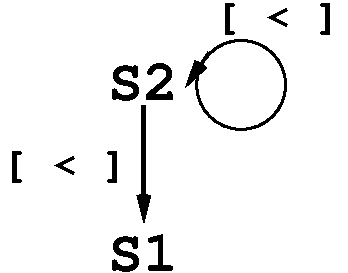
\includegraphics[height=15ex]{img/LoopDistr.pdf}
\end{center}

\noindent and it exhibits two strongly-connected components:
one formed by statement $S_2$ and one formed by statement $S_1$.
Loop distribution results in the following restructured code:
\begin{lstlisting}[mathescape=true]
for (int i = 2; i < N; i++)
  $S_2:$  B[i] = B[i-1] ...
for (int i = 2; i < N; i++)
  $S_1:$  A[i] = B[i-2] ...
\end{lstlisting}
in which, according to the graph order, the loop corresponding to
statement $S_2$ appears before the one corresponding to statement
$S_1$. Note that this does not match the program order of statements
$S_1$ and $S_2$ in the original program. Also note that the first loop
is \emph{not} parallel because the SCC consisting of $S_2$ has a
(dependency) cycle, but the second loop is parallel because the SCC
corresponding to $S_1$ does not have cycles.

If a loop is parallel then it can be straightforwardly distributed
across its statements in program order because:
\begin{itemize}
\item by \cref{Dep-Cycle}, the loop dependency graph has no cycles and
  thereby each statement is a strongly connected component;
\item the program order naturally respects all dependencies.
\end{itemize}

\begin{corollary}[Parallel loop distribution]\label{Par-Loop-Distr}
  A parallel loop can be directly distributed across each one of its
  statements. The resulting loops appear in the same order in which
  their corresponding statements appear in the original loop.
\end{corollary}

\subsection{Array expansion}
\label{sec:array-expansion}

Finally, it remains to demonstrate array expansion, mentioned
in the fourth bullet of \cref{Loop-Distrib}. Assume the slightly
modified code:
\begin{lstlisting}[mathescape=true]
float tmp;
for (int i = 2; i < N; i++) {
  $S_1:$  tmp  = 2 * B[i-2];
  $S_2:$  A[i] = tmp;
  $S_3:$  B[i] = tmp + B[i-1];
}
\end{lstlisting}
Statements $S_1$ and $S_3$ are in a dependency cycle, because
there is a dependency $S_3\to S_1$ with direction \texttt{<} caused
by the write to and the read from array \texttt{B}, and a dependency
$S_1\to S_3$ with direction \texttt{=} caused by \texttt{tmp}.
Statement $S_2$ is not in a dependency cycle, but there is a
dependency $S_1\to S_2$, and hence its distributed loop
should follow the distributed loop containing $S_1$ and $S_3$.
If we do not perform array expansion, the distributed code:

\pagebreak
\begin{lstlisting}[mathescape=true]
float tmp;
for (int i = 2; i < N; i++) {
  $S_1:$  tmp  = 2 * B[i-2];
  $S_3:$  B[i] = tmp + B[i-1];
}
for (int i = 2; i < N; i++) {
  $S_2:$  A[i] = tmp;
}
\end{lstlisting}
\noindent does not respect the semantics of the original program
because the second loop uses the same value of \texttt{tmp}---the one
set by the last iteration of the first loop---while the original loop
writes and then reads a different value of \texttt{tmp} for each
iteration. We fix this by performing array expansion for \texttt{tmp},
which means that we must expand it with an array dimension equal to
the loop count and replace its uses with corresponding indexing
expressions of the expanded array.  This results in the following
\emph{correct} code:

\begin{lstlisting}[mathescape=true]
float tmp[N];
for (int i = 2; i < N; i++) {
  $S_1:$  tmp[j]  = 2 * B[i-2];
  $S_3:$  B[i] = tmp + B[i-1];
}
for (int i = 2; i < N; j++) {
  $S_2:$  A[i] = tmp[j];
}
\end{lstlisting}

Array expansion requires us to normalise the loop first---this means
rewriting the loop such as its index starts from $0$ and increases by
$1$ each iteration. This is why we have not written our example as
\lstinline{do i = 2, N+1}.

\section{Eliminating false dependencies (WAR and WAW)}
\label{sec:false-dep-elim}

Anti and output dependencies are often referred to as \emph{false}
dependencies because they can be eliminated in most cases by copying
or privatisation operations:
\begin{itemize}
\item Cross-iteration anti dependencies (WAR) typically
  correspond to a read from some original element of
  the array---whose value was set before the start of
  the loop execution---followed by an update to that
  element in a later iteration.  As such, this dependency
  can be eliminated by copying (in parallel) the target
  array before the loop and rewriting the offending
  read access inside the loop such that it refers
  to the copy of the array.

\item Cross-iteration output dependencies (WAW) can be
  eliminated by a technique named privatisation (or renaming),
  whenever it can be determined that {\em every read access}
  from a scalar or array location {\em is covered by an
    update} to that scalar or memory location that was
  previously performed {\em in the same iteration}.
  Semantically, privatisation moves the declaration of the
  offending variable inside the loop, because it has been
  already determined that the read/used value was produced
  earlier in the same iteration.

\item Reasoning based on direction vectors is limited to
  relatively simple loop nests; for example it is difficult
  to reason about privatisation by means of direction vectors.
\end  {itemize}

\subsection{Eliminating WAR dependencies by copying}

Consider the simple C code below which rotates an array in the right
dimension by one:

\begin{lstlisting}[mathescape=true]
float tmp = A[0];
for (int i=0; i<N-1; i++) {
    A[i] = A[i+1]; // $S_1$
}
A[N-1] = tmp;
\end{lstlisting}

The loop exhibits a cross-iteration anti dependency (WAR) $S_1\to S_1$
(with direction vector $\texttt{[<]}$), and, as such, it is not safe
to execute it in parallel. However, one can observe that the reads
from \texttt{A} inside the loop correspond to the original elements of
\texttt{A} before the loop, because they are rewritten in a later
iteration.  As such one can perform a copy of \texttt{A} before the
loop, and replace the read access inside the loop to operate on the
copy of array \texttt{A}. This preserves the original loop semantics
and results in a parallel loop because the read and write accesses
operate on different arrays, hence a dependency cannot occur. For
example, using OpenMP:

\begin{lstlisting}[mathescape=true]
float Acopy[N];
#pragma omp parallel for
for (int i=0; i<N; i++) {
    Acopy[i] = A[i];
}
tmp = A[0];
#pragma omp parallel for
for (int i=0; i<N-1; i++) {
    A[i] = Acopy[i+1];
}
A[N-1] = tmp;
\end{lstlisting}

Note that in a real program, we would allocate the \texttt{Acopy}
array with \texttt{malloc()} rather than creating a potentially very
large stack allocation.

\subsection{Eliminating WAW dependencies by privatisation}

Consider the contrived and ugly looking C code below:

\begin{lstlisting}[mathescape=true]
int A[M];
for (int i=0; i<N; i++){
  for (int j=0, j<M; j++) { // writes slice A[0:M-1]
    A[j] = (4*i+4*j) % M;   // $S_1$
  }
  for (int k=0; k<N; k++) { // reads A[j] where j$\in${0,$\ldots$M-1}
                            // because % denotes modulus op
    X[i][k] = X[i][k-1] * A[ A[(2*i+k)%M] % M];      // $S_2$
  }
}
\end{lstlisting}

Analysing the cross-iteration dependencies of the outer loop,
one can observe that there are frequent output dependencies
$S_1\to S_1$ of all directions (\texttt{*}), because, in
essence, all elements of \texttt{A} at indices $0\ldots M-1$
are (over)written in each iteration of the outer loop.
This also causes frequent cross-iteration WAR and RAW
dependencies between $S_1$ and $S_2$ of all directions
\texttt{*} because $S_2$ reads some of the values of
\texttt{A} which are written in $S_1$. The read access
is also statically unanalysable because the index
into \texttt{A} depends on a value of \texttt{A} (i.e.,
it is an indirect-array access \texttt{A[ A[...] ]}).

It would thus seem that this is a hopeless case and parallel
execution is a pipe dream. Not so! Actually the rationale
of how to transform the outer loop into a parallel one
is quite simple.  One may observe that each iteration of
the outer loop writes the same indices of \texttt{A}, namely
the ones belonging to the closed integral interval
\texttt{[0,M-1]}.   One may also observe that $S_2$ reads
from \texttt{A} elements whose indices necessarily belong to
\texttt{[0,M-1]}---due to the two modulus-\texttt{M} operations.
As such, one may conclude that any value
read in $S_2$ must have been produced in the same iteration
of the outer loop (in the inner loop enclosing $S_1$).

It follows that it is safe to rewrite the loop in the
following way:
\begin{enumerate}
\item Declare a new variable \texttt{A'} of the same dimensions as
  \texttt{A} just inside the outer loop (or equivalently perform array
  expansion of array \texttt{A'} with a new outer dimension of size
  \texttt{N}).
\item Replace all the uses of \texttt{A} in the outer loop by uses of
  \texttt{A'}.  The resulting loop is safe to execute in parallel
  because there can be no dependencies on \texttt{A'} since each
  iteration uses a different array \texttt{A'}.
\item As a last step, after the parallel execution of the loop
  terminates, one must copy (in parallel) the elements produced by the
  last iteration of the outer loop (i.e., \texttt{A'[0,$\ldots$][M-1]}
  back to \texttt{A}.
\end{enumerate}

The parallel OpenMP code that implements these steps is
presented below:

\begin{lstlisting}[mathescape=true]
int A[M];
#pragma omp for lastprivate(A)
for (int i=0; i<N; i++) {
    for(int j=0, j<M; j++) {
        A[j] = (4*i+4*j) % M;
    }
    for(int k=0; k<N; k++) {
        X[i][k]=X[i][k-1] * A[ A[(2*i+k) % M] % M];
    }
}
\end{lstlisting}

Declaring array \texttt{A} as private (by using the clause
\texttt{private(A)}) would result in semantically performing steps (1)
and (2) above. Using the \texttt{lastprivate(A)} clause instructs the
OpenMP compiler to also perform step (3)---to copy back the
privately-maintained result of \texttt{A} of the last executing
iteration into the globally-declared array \texttt{A}.

Please also note that the OpenMP execution will not allocate
a new \texttt{A'} for each iteration of the outer loop---this is
actually equivalent to performing array expansion which is also
applicable here---but instead it will {\em allocate a copy of
  \texttt{A} for each active thread}, thus significantly reducing
the memory footprint and/or the number of (de)allocations.

Privatisation can be applied whenever one can prove that every read
access in an iteration is covered by a previously-performed write
access in the same iteration.  Privatisation can be implemented by
performing either array expansion or moving the declaration of the
target variable from outside to inside the loop. However, it saves
memory to allocate the private copy per active thread rather than per
iteration, which is what OpenMP is doing.

\section{Loop stripmining, block and register tiling}
\label{sec:strip-tiling}

This section discusses several simple transformations that are going
to be combined in various ways to optimise locality of reference (both
temporal and spatial locality).

\textbf{\em Stripmining} refers to the following transformation,
which is always safe to apply:
\begin{lstlisting}[mathescape=true]
for(int i = 0; i<N; i++) {      for(int ii = 0; ii<N; ii+=T){
  iteration body            $\Rightarrow$    for(int i=ii, i<min(ii+T,N); i++)
}                                     iteration body
                                } }
\end{lstlisting}
In essence, a normalized loop is split into a perfect nest of two
loops, in which the first loop goes with stride \texttt{T}, and
the second one goes with stride \texttt{1}. Please notice that the
resulting loop nest executes the same number of statements and
in the same order as the original loop.

\textbf{\em Block tiling} refers to the transformation that
stripmines several consecutive innermost loops in a
perfect loop nest---named $l_{k+1}\ldots l_{k+n}$---and then
interchanges inwards the resulting loops of stride $1$.
The transformation is valid/safe if in the original program
it is safe to interchange any of the loops
$l_{k+i},~i\in\{1,\ldots,n-1\}$ in the innermost position.
For example, the code below demonstrates block tiling a perfect
loop nest of depth two:
\begin{lstlisting}[mathescape=true]
for(i = 0; i<N; i++) {      for(ii=0; ii<N; ii+=T1) {
  for(j = 0; j<M; j++) {      for(jj=0; jj<M; jj+=T2) {
    iteration body       $\Rightarrow$     for(i=ii; i<min(ii+T1,N); i++) {
  }                               for(j=jj; j<min(jj+T2,M); j++) {
}                                   iteration body
                            } } } }
\end{lstlisting}

\textbf{\em Unroll and jam} refers to the transformation that partially
unrolls one or more of the outer loops in a perfect nest and then
fuses (``jams'') the resulting loops. Equivalently, one can stripmine
an outer loop, then interchange (distribute) it in the innermost
position, then completely unroll it. The transformation is aimed at
decreasing the number of memory loads and stores by storing to and
reusing values from registers, and thus it is applied when the
original loop nest contains data references that allow for temporal
reuse---e.g., their indexes are invariant to some of the loops
in the nest.
Due to this, it is also known as ``{\em register tiling}''.
We demonstrate the transformation on the matrix-matrix
multiplication code below:
\begin{lstlisting}[mathescape=true]
for(i=0; i<N; i++) {
  for(j=0; j<M; j++) {
    float c;
    c = 0.0;
    for(k=0; k<N; k++) {
      c += A[i][k] * B[k][j];
    }
    C[i][j] = c;
  }
}
\end{lstlisting}

The plan is to stripmine the loop of index \texttt{j} by a tile of
size $2$, and to interchange it to the innermost position, while
performing the necessary loop distribution and array expansion:
\begin{lstlisting}[mathescape=true]
for(i=0; i<N; i++) {
  for(jj=0; jj<M; jj+=2) {
    float cs[2];
    for(j=jj; j<min(jj+2,M); j++) {
        cs[j-jj] = 0.0;
    }
    for(k=0; k<N; k++) {
      for(j=jj; j<min(jj+2,M); j++) {
        cs[j-jj] += A[i][k] * B[k][j];
    } }
    for(j=jj; j<min(jj+2,M); j++) {
        C[i][j] = cs[j-jj];
    }
} }
\end{lstlisting}
One can observe that the access \texttt{A[i][k]} is invariant to its
immediately contained loop of index \texttt{j} and thus it can be hoisted
outside it and saved into a register. Then the loops of index \texttt{j}
can be unrolled, and array \texttt{cs} can be scalarized as well:
\begin{lstlisting}[mathescape=true]
for(i=0; i<N; i++) {
  for(jj=0; jj<M; jj+=2) {
    float c1, c2;
    if (jj   < M) c1 = 0.0;
    if (jj+1 < M) c2 = 0.0;
    for(k=0; k<N; k++) {
      float a;
      a = A[i,k];
      if (jj   < M) c1 += a * B[k][jj  ];
      if (jj+1 < M) c2 += a * B[k][jj+1];
    }
    if (jj   < M) C[i][jj  ] = c1;
    if (jj+1 < M) C[i][jj+1] = c2;
} }
\end{lstlisting}
In the resulted code, the accesses to the elements of \texttt{A} have
been halved.   We can similarly apply unroll and jam for the loop
of index \texttt{i} with a tile size equal to \texttt{3}. This will cut down
the accesses to \texttt{B} by a factor of $3$. The resulted code
is shown in \cref{fig-unroll-jam}.

\begin{figure}
\begin{lstlisting}[mathescape=true]
for(ii=0; ii<N; ii+=3) {
  for(jj=0; jj<M; jj+=2) {

    float c11, c12, c21, c22, c31, c32;

    if (ii   < N && jj   < M) c11 = 0.0;
    if (ii+1 < N && jj   < M) c21 = 0.0;
    if (ii+2 < N && jj   < M) c31 = 0.0;
    if (ii   < N && jj+1 < M) c12 = 0.0;
    if (ii+1 < N && jj+1 < M) c22 = 0.0;
    if (ii+2 < N && jj+1 < M) c32 = 0.0;

    for(k=0; k<N; k++) {

      float a1, a2, a3, b1, b2;

      if (ii   < N) a1 = A[ii  ][k];
      if (ii+1 < N) a2 = A[ii+1][k];
      if (ii+2 < N) a3 = A[ii+2][k];
      if (jj   < M) b1 = B[k   ][jj];
      if (jj+1 < M) b2 = B[k   ][jj+1];

      if (ii   < N && jj   < M) c11 += a1 * b1;
      if (ii+1 < N && jj   < M) c21 += a2 * b1;
      if (ii+2 < N && jj   < M) c31 += a3 * b1;
      if (ii   < N && jj+1 < M) c12 += a1 * b2;
      if (ii+1 < N && jj+1 < M) c22 += a2 * b2;
      if (ii+2 < N && jj+1 < M) c32 += a3 * b2;
    }

    if (ii   < N && jj   < M) C[ii  ][jj  ] = c11;
    if (ii+1 < N && jj   < M) C[ii+1][jj  ] = c21;
    if (ii+2 < N && jj   < M) C[ii+2][jj  ] = c31;
    if (ii   < N && jj+1 < M) C[ii  ][jj+1] = c11;
    if (ii+1 < N && jj+1 < M) C[ii+1][jj+1] = c21;
    if (ii+2 < N && jj+1 < M) C[ii+2][jj+1] = c31;
  }
}
\end{lstlisting}
  \caption{Result of unroll-and-jam applied to matrix-matrix
    multiplication, where the first and second outer loops were tiled
    with sizes $3$ and $2$, respectively. The number of accesses to
    \texttt{A} and \texttt{B} has been reduced by a factor of
    $2\times$ and $3\times$, respectively, at the expense of
    introducing some conditional statements.}
  \label{fig-unroll-jam}
\end{figure}

%%% Local Variables:
%%% mode: latex
%%% TeX-master: "notes"
%%% End:
